\documentclass[a4paper,12pt]{report}
\usepackage{alltt, fancyvrb, url}
\usepackage{graphicx}
\usepackage[utf8]{inputenc}
\usepackage{float}
\usepackage{hyperref}
\usepackage[italian]{babel}
\usepackage[italian]{cleveref}
\title{Relazione su "Daidokoro" \\ Elaborato per il corso di Basi di Dati}

\author
{
    Matteo Giorgini - 0001136576 \\
    Tommaso De Tommaso - 0001077338 \\
    Edoardo Scorza - 0001077424 \\
}
\date{\today}
\begin{document}
\maketitle
\tableofcontents

\chapter{Analisi dei requisiti}
Si vuole realizzare un database a supporto di un social network di ricette.
Questo dovrà immagazzinare dati relativi agli utenti registrati, alle ricette pubblicate, gli ingredienti disponibili, i valori nutrizionali, la categoria nutrizionale, i preferiti, le valutazioni, le collezioni e gli obiettivi.

\section{Intervista}
Si vuole tenere traccia degli \textbf{utenti} registrati salvandone il loro username, la foto profilo, l'email, la password, l'esperienza ed il livello, che vengono usati per premiare un maggiore utilizzo del social network, inoltre viene generato un codice univoco per identificarlo. Un utente, una volta registrato, potrà effettuare l'accesso ed utilizzare il social network osservando le ricette altrui, aggiungendole ai preferiti, salvandole in collezioni o in diete e valutandole con un voto ed un commento. Inoltre l'utente potrà pubblicare le proprie ricette e sbloccare obiettivi.
Una \textbf{ricetta} è caratterizzata da un nome, una foto, una descrizione, una difficoltà e un tempo di realizzazione indicativo, oltre agli ingredienti che la compongono ed i passi necessari a prepararla.
Un \textbf{ingrediente} è caratterizzato da un nome, una descrizione, dai suoi valori nutrizionali e dalla categoria nutrizionale a cui appartiene.
Una \textbf{collezione} è caratterizzata da un nome, una descrizione, una data e le ricette che ne fanno parte. Lo stesso vale per una \textbf{dieta}, tuttavia questa deve anche aderire ad una categoria nutrizionale specifica, vincolando le ricette contenute. Ad esempio, la dieta per i celiaci aderirà alla categoria nutrizionale della celiachia e potrà comprendere solo ricette con ingredienti compatibili.
Un \textbf{obiettivo} è caratterizzato da un nome, una descrizione e dalla quantità di esperienza da dare all'utente una volta sbloccato.

[ SPIEGAZIONE SU COME SBLOCCARE E COSA LIMITANO GLI OBIETTIVI ]

[ ANALISI DELLE VALUTAZIONI ]

\section{Ambiguità}
Secondo sottocapitolo
\section{Definizioni}
Secondo sottocapitolo


\chapter{Progettazione concettuale}
Per la progettazione concettuale abbiamo considerato diverse cose,
tra cui, la organizzazione della applicazione e le capacità degli utenti,
in primis, la app è di tipo client-server, quindi il database è unico e
possiede tutti i dati del "ecosistema"(client e server), gli utenti sono potenzialmente tanti
e hanno un frequente accesso al database, motivo per il cui i dati sono
frammentati, separati in varie parti, per evitare un accesso non essenziale a grandi quantità di dati, e ridurre il carico sul database.    
\section{Schema scheletro}
\begin{figure}[H]
    \centering
    \includegraphics[width=0.8\textwidth]{image.png}  
    \label{fig:example}
\end{figure}
La prima versione dello schema evidenzia gli elementi chiave 
che costruiscono le informazioni su cui si basa la applicazione:
\begin{itemize}
    \item Utente
    \item Ricetta
    \item Valutazione
    \item Ingrediente
    \item Dieta
\end{itemize}

\section{Raffinamenti proposti}
Analizzando meglio la possibile esperienza dell'utente
sono molte le possibili aggiunte, abbiamo cercato
dunque di rendere il database completo senza complicarlo eccessivamente:
\subsection{Dieta}
La dieta, corrisponde alla possibilità di raggruppare ricette
per rendere più significativo il significato di essa abbiamo deciso di 
imporre dei limiti, come la categoria, che limita la tipologia di ricette 
inseribili, la creazione di essa è permessa all'utente solo dopo aver sbloccato un determinato obiettivo.
\subsection{Collezione}
Per non limitare le possibilità dell'utente abbiamo deciso di creare 
una variante più generale della dieta, la collezione
essa permette di salvare ricette indiscriminatamente.
\subsection{Obiettivo}
Per Dare più autorevolezza agli utenti esperti e
filtrare utenti "troll" abbiamo deciso di implementare dei requisiti,
per fare delle diete bisogna aver sbloccato un obbiettivo, 
cosi per le critiche
\subsection{Valutazione}
Per le valutazioni abbiamo optato su 2 tipologie
valutazione e critica, la prima consiste in un voto
numerico, assegnabile da un utente generico, il secondo è una critica
che aggiunge il commento, questa limitata da un obbiettivo.


\section{Schema Concettuale}
Il risultato finale è questo schema:
\begin{figure}[H]
    \centering
    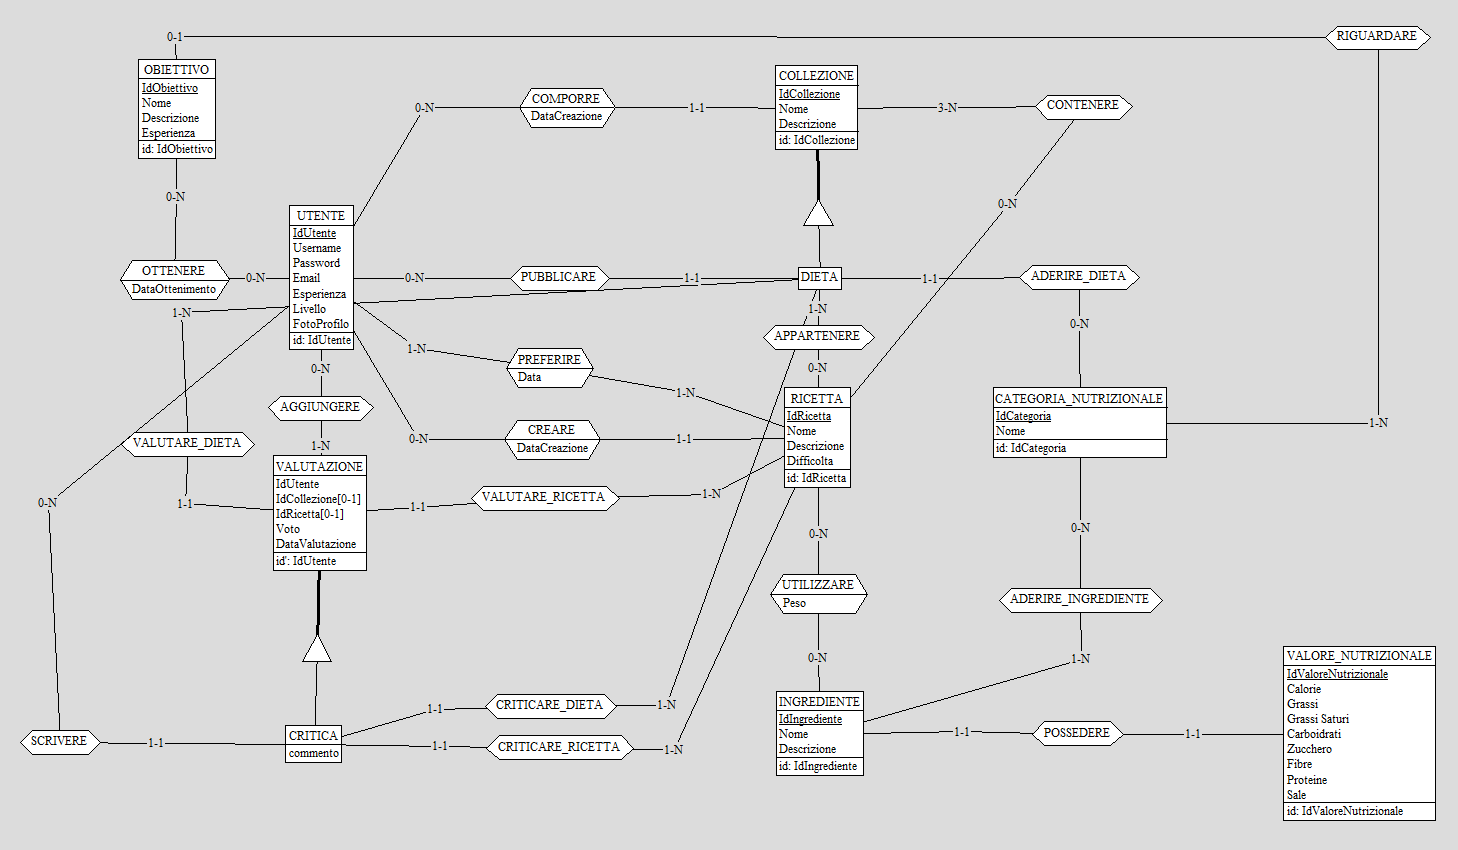
\includegraphics[width=0.9\linewidth]{schema-concettuale.png}
    \label{fig:enter-label}
\end{figure}

\subsection{Valutazione}
Per rappresentare le valutazioni e critiche
abbiamo optato per una gerarchia.
\begin{figure}[H]
    \centering
    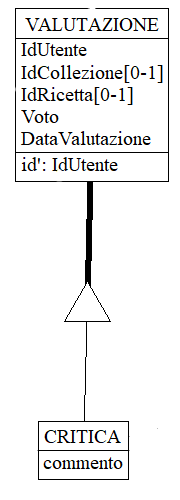
\includegraphics[width=0.2\linewidth]{valutazione-concettuale.png}
    \label{fig:enter-label}
\end{figure}
\subsection{Ingrediente}
Per rappresentare gli ingredienti abbiamo preferito separarlo in due entità, ingrediente e valori nutrizionali
\chapter{Progettazione logica}
capitolo logica
\section{Volume dei dati}
Secondo sottocapitolo
\section{Operazioni principali e frequenza}
Secondo sottocapitolo
\section{Tabelle degli accessi}
Secondo sottocapitolo
\section{Raffinamento schema}
Secondo sottocapitolo
\section{Analisi rindondanze}
Secondo sottocapitolo
\section{Traduzione di entità e relazioni in associazioni}
Secondo sottocapitolo
\section{Schema relazionale finale}
Secondo sottocapitolo
\section{Traduzione delle operazioni in query SQL}
Secondo sottocapitolo


\chapter{Progettazione applicazione}
capitolo logica
\section{Piattaforma di sviluppo}
sezione
\section{Architettura}
sezione
\end{document}
